\section{定位与导航}

\subsection{规划}
路径规划使用\lstinline{ros-planning}中的 \lstinline{navigation} 来进行全局路径规划以及局部路径规划，全局路径规划使用 A star 搜索算法来得到机器人底盘到目标点的全局路径，局部路径使用 Timed Elastic Band算法来得出局部范围内的路径，并且向全局规划得出的路径收敛。
由于哨兵需要在三个巡逻区中进行巡航，而其中的两个巡逻区需要机器人上坡才能到达，然而直接采用雷达的点云信息，\lstinline{costmap_2d} 会根据斜坡点云生成障碍层，使其被视为障碍物，因此我们需要用于路径规划的点云能够根据坡度来产生相应的变化，我们采取了两种地图工具来实现
\paragraph{octomap}
我们使用原始点云来构建 octomap ，滤除高于机器人限高的点云，同时从点云数据中检测和忽略地平面，从而清除掉地面上的所有点云，不会将地面作为障碍物插入地图中，因此我们可以调整检测地面的角度阀值，来判断对应的斜坡是否是地图中可以通过的区域。
\paragraph{elevation\_map}
除了尝试 octomap 来处理点云，我们还通过开源包 \lstinline{elevation_mapping} 构建场地的高程图来得到三维地图信息，从而判断以及滤除地面信息，通过测试，我们发现构建出的 elevation\_map 比 octomap 更加适合，因此我们最后采用 \lstinline{elevation_mapping} 来处理点云并用于规划。

\subsection{定位}
为了保证从世界坐标系到机器人的底盘坐标系 \lstinline{map -> base_link} 的准确性，我们这部分坐标转换关系分成了如下两部分分别修复。
\subsubsection{全局定位}
全局定位需要维护的是　\lstinline{map -> odom}　的坐标变换关系，我们采用两种方式来修复 \lstinline{map -> odom} ，第一种是识别场地的标签，第二种是通过雷达机器人发布的机器人位姿信息，两种方式进行互补以确定 \lstinline{ map } 到 \lstinline{ odom } 的坐标转换。
\paragraph{场地标签识别}
哨兵在场地上需频繁移动，而在一些特殊的情况下，哨兵可能会遇到一些障碍，导致传感器无法准确地获取位置信息，从而在后续的路径规划中偏离预定的目标点。为此，我们可以利用赛场上的视觉标签，通过哨兵的相机来检测这些标签的位置和朝向，并借此修复哨兵在场景中的位置信息。这种做法易于实现的同时，可以获得比传感器本身更精确的位置信息。

\paragraph{传统视觉算法方案} 我们采取的传统视觉算法方案如下，其在光照变化不大时，能够保证修复结果误差小，效果良好。

\subparagraph{图像阈值分割}
由于单目相机的限制，在哨兵巡航过程中我们不希望其根据远处的标签来进行修复，经实验测试这会导致位姿解算时姿态发生较明显的抖动而导致修复定位的效果较差，所以我们期望其可识别标签的距离范围在3-5m以内。故我们采用大津法对图像进行前后景的分割，该方法的基本思想是根据选取的阈值将图像分为目标和背景两个部分，计算像素的灰度值对应的最大类间方差值，将类间方差值取最大时对应的阈值作为最佳阈值。定义：目标阈值为$t$，前景为$f$，背景为$b$，当前阈值为$k$，当前阈值为$k$时像素被分为前景的概率为$p_f\left(k\right)$，当前阈值为k时像素被分为背景的概率为$p_b\left(k\right)$，前景像素的平均灰度为$m_f\left(k\right)$，背景像素的平均灰度为$m_b\left(k\right)$。求方差的公式便可以表示为：
\begin{equation}
    \sigma^2 = p_f(k)p_b(k)(m_f(k) - m_b(k))^2
\end{equation}
求得最大方差时所对应的$t$便是目标阈值

\subparagraph{形态学处理}
在形态学方面，我们主要是想要通过开操作来对图像进行处理以达到去除目标边界的噪点而让目标边界的纹理特征更加明显的目的。定义$element$表示结构元，$(x,y)$为锚点$O$的位置，$x'$和$y'$为结构元值为1的像素相对锚点$O$的位置偏移，$src$表示原图，$dst$表示结果图。膨胀运算用公式符号表示为:$f \oplus s$，其公式可以表示如下：
\begin{equation}
    dst(x,y) = \max\limits_{(x',y'):element(x',y')\ne0}src(x+x',y+y')
\end{equation}
腐蚀运算用公式符号表示为：$f \ominus s$，其公式可以表示如下：
\begin{equation}
    dst(x,y) = \min\limits_{(x',y'):element(x',y')\ne0}src(x+x',y+y')
\end{equation}
对图像进行开运算相当于先进行腐蚀再进行膨胀，其公式可以表示为：$f \circ s=(f \ominus s) \oplus s$

\subparagraph{多边形拟合}
通过对提取的轮廓进行采用Douglas-Peuker算法因其可以处理大量冗余的几何数据点，可以在很大程度上保留几何形状的骨架的原因，可以用来判断轮廓的形状，以在所提取特征集合中取出视觉标签的轮廓。该算法的基本思路为将待处理曲线的首末点虚连一条直线,求所有中间点与直线的距离,并找出最大距离值$dmax$ ,用$dmax$与抽稀阈值$threshold$相比较：
若$dmax < threshold$，这条曲线上的中间点全部舍去;
若$dmax \geq threshold$，则以该点为界，把曲线分为两部分,对这两部分曲线重复上述过程，直至所有的点都被处理完成。

\subparagraph{图像矩计算}
矩在统计学意义上，表示为：一个随机变量的分布，可以由1到无穷阶的矩唯一确定，每一阶矩都从某个角度去描述了这个随机变量分布的性质。那么也就是说每一阶矩都对应一个概率分布。定义$I(x,y)$是图像在像素$(x,y)$处的像素值，图像的几何矩计算公式如下：

\begin{equation}
    m_{ji} = \sum_{x,y}I(x,y)x^jy^i
\end{equation}

通过图像的一阶矩和零阶矩可以计算质心，计算公式如下：
\begin{equation}
    \overline{x} = \frac{m_{10}}{m_{00}},\overline{y} = \frac{m_{01}}{m_{00}},
\end{equation}
而中心矩计算公式为：
\begin{equation}
    mu_{ji} = \sum_{x,y}I(x,y)(x - \overline{x})^j(y - \overline{y})^i
\end{equation}
归一化几何矩的计算公式则为：
\begin{equation}
    nu_{ij} = \frac{mu_{ij}}{m_{00}^(1+\frac{i+j}{2})}
\end{equation}

\subparagraph{Hu矩与元素辨别}
根据在1962年“Visual Pattern Recognition by Moment Invariants”论文所提，Hu矩可以被用来获得相对于特定变换的不变性。该不变性可以让我们在特征轮廓发生平移、缩放和旋转情况下稳定的辨认出特特征，其前提是在连续域中，因为在离散域中缩放和旋转都没有很好地定义，其不变性在此时更趋向于近似不变。Hu矩的计算公式由归一化几何矩得来，公式如下：

\begin{equation}
\begin{aligned}
    &I_1 = nu_{20} + nu_{02} \\
    &I_2 = (nu_{20} - nu_{02})^2 + 4nu_{11}^2 \\
    &I_3 = (nu_{30} - 3nu_{12})^2 + (3nu_{21} - nu_{03})^2 \\
    &I_4 = (nu_{30} + nu_{12})^2 + (nu_{21} + nu_{03})^2 \\
    &I_5 = (nu_{30} - 3nu_{12})(nu_{30} + nu_{12})\\
    &* [(nu_{30} + nu_{12})^2 - 3(nu_{21} + nu_{03})^2] \\
    &+ (3nu_{21} - nu_{03})(nu_{21} + nu_{03}) \\
    &*[3(nu_{30} + nu_{12})^2 - (nu_{21} + nu_{03})^2] \\
    &I_6 = (nu_{20} - nu_{02})[(nu_{30} + nu_{12})^2 \\
    &- (nu_{21} + nu_{03})^2] + 4nu_{11}(nu_{30} + nu_{12})(nu_{21} + nu_{03}) \\
    &I_7 = (3nu_{21} - nu_{03})(nu_{30} + nu_{12})[(nu_{30} + nu_{12})^2 - 3(nu_{21} + nu_{03})^2] \\
    &- (nu_{30} - 3nu_{12})(nu_{21} + nu_{03})[3(nu_{30} + nu_{12})^2 - (nu_{21} + nu_{03})^2]
\end{aligned}
\end{equation}
对于一个特定的物体轮廓，其Hu矩是确定的，故而我们采取此方法用于辨别视觉标签的内容，来使我们的哨兵“知道自己看到的是哪一个标签，从而知道自己当前的位置”。
我们定义相似程度的概念，用于计算两轮廓之间的相似程度。假设A，B各自为两轮廓，令$S(A,B)$为相似程度的量化值，其越小，两轮廓越相似，令$m_i^A = sign(I_i^A)log(I_i^A),m_i^B = sign(I_i^B)log(I_i^B)$,相似程度计算公式如下：
\begin{equation}
    S(A,B) = \sum_{i=1...7}|m_i^A - m_i^B|
\end{equation}

\subparagraph{八连通域提取标签信息}
对于标签内的字母与数字，如果想要提取其轮廓，仅仅靠外轮廓提取算法是很难实现获得完整特征的。此处我们选择使用八连通域跟踪算法进行字母与数字的特征提取。八连通域跟踪算法基本思想是，遍历图像找到第一个非零像素点，设这个点为起始点$x$，顺时针查找该点八邻域内遇到的第一个非零像素点$x'$（点$x'$也为边界点）。令$x=x'$，再进行邻域内的顺时针查找，查找的起点为刚刚$x$到$x'$过程中$x'$前一个零点，直到没有扫描到非零像素点，则认为找到一个连通域，对其记录标签和相应信息。(详见\ref{fig:视觉标签_设计方案-1})

\begin{figure}[H]
    \centering
    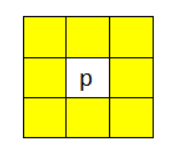
\includegraphics[width=0.4\columnwidth]{figure/设计方案/定位与导航/8Connect.png}
    \caption{直观的八连通域示意图}
    \label{fig:视觉标签_设计方案-1}
\end{figure}

八邻域算法可以很高效且容易地提取到标签字母和数字，能够保留其完整特征，易于标签类别的辨别，提取效果如\figref{fig:视觉标签_设计方案-2}所示。

\begin{figure}[H]
    \centering
    
\includegraphics[width=0.3\columnwidth]{figure/设计方案/定位与导航/Tagdisplay.jpg}
    \caption{八连通域跟踪算法提取效果}
    \label{fig:视觉标签_设计方案-2}
\end{figure}

\subparagraph{N点透视位姿求解}~~在辨别完标签内容后，便可以进行标签的位姿估计。因为标签尺寸固定且单目相机的限制，使用N点透视位姿求解无疑是最具“性价比”的方法。我们采用Levenberg-Marquardt下降法来对构建的重投影误差进行优化，因我们所取的点都在视觉标签的一个平面上，所以位姿的获取来自于单应性矩阵的SVD分解。经过优化迭代后，便可以获得相机与视觉标签之间的位姿，提供给全局地图修复使用。

\subparagraph{卷积神经网络} 由于哨兵高速运动的原因，深度学习模型的轻量性极为重要，而又由于位姿估计需要准确的点对，我们将普通的基于水平框(xywh)而进行的目标检测算法改成了基于四个点(x1/2/3/4,y1/2/3/4)的任意四边形目标检测算法。其能在场景不确定性较大的情况下依然能够实现较好的需求效果。

网络主要组成结构采取Enhanced ShuffleNet 作为backbone，其主要由ES block组成，如\figref{fig:视觉标签_设计方案-3}所示。

\begin{figure}[H]
    \centering
    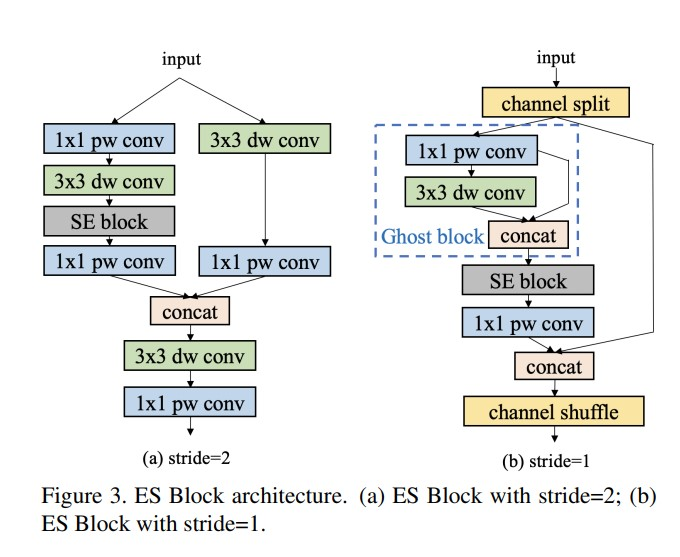
\includegraphics[width=0.5\columnwidth]{figure/设计方案/定位与导航/ES_block.jpg}
    \caption{ES block}
    \label{fig:视觉标签_设计方案-3}
\end{figure}

由上可见，其必备的组成部分是与MobileNetV3相似的SE模块和depthwise/pointwise卷积模块。在stride = 1时，其中纳入了由GhostNet作者所提出的novel Ghost模块，其主旨是以较少的参数生成更多的特征图以提高模型的学习能力。Channel shuffle可以提供通道之间信息交换的能力，但是会导致学习融合特征的能力减弱，因此采取depthwise/pointwise卷积模块来融合不同通道的信息以弥补上述缺点。在neck层，我们采取CSP-PAN的网络结构来提取多尺度特征。

\subparagraph{样本分配}
对于Head中的样本分配，我们采取在TOOD论文中所提到的TAL算法并加以修改，我们利用其结合分类与定位的分配思想，将定位权重计算方法改为以顶点距和质心距为基础的的指数运算，能够在任意四边形下的目标检测场景达到不错的效果。

\subparagraph{损失函数}
而对于较为重要的损失函数，我们采取了一种计算两多边形之间距离的方法。其中心思想在于构建一个多边形的顶点与另一个多边形的所有边之间的三角形，其面积可作为衡量的标准，这种方法的具有显而易见的连续性和可微性的。容易理解的一个思想是：若某个点存在于多边形内，其与多边形顶点之间所构成的三角形面积和应等于整个多边形的面积（这也是我们在样本分配时采取的思想），那么我们作如下定义：存在多边形$A$，顶点数为$n$，多边形$B$，顶点数为$m$，$S_{PPA}$作为$A$各顶点到$B$上各边面积的和，则距离可以表述为$distance = (\frac{1}{n}S_{PPA} - S_B) + (\frac{1}{m}S_{PPB} - S_A) $

\subparagraph{哨兵位姿修复}
通过相机获取标签到相机的变换矩阵${}^{tag}T_{cam} $后，我们可以根据相机到哨兵基坐标系的变换矩阵${}^{cam}T_{base} $,通过矩阵变换公式：
\begin{equation}
    {}^{tag}T_{base}={{}^{tag}T_{cam} } {}^{cam}T_{base}  
\end{equation}
得到标签相对与哨兵的变换矩阵${}^{tag}T_{base}$；再通过已知的地图到对应标签的变换矩阵${}^{map}T_{tag}$,经过矩阵变换后得到当前哨兵相对地图的位置${}^{base}T_{map}$。

为了兼顾定位定姿算法的鲁棒性与时效性，我们不会直接使用${}^{base}T_{map}$替换,而是将多帧图像得到的${}^{base}T_{map}$取移动平均，最后计算出世界坐标系到里程计坐标系的变换关系：
\begin{equation}
    {}^{odom}T_{map}={}^{odom}T_{base} {}^{base}T_{map}
\end{equation}
 计算出当前哨兵里程计\lstinline{odom}相对与地图map的正确位姿。
 

受限于相机性能与现场光照条件，通过视觉算法计算出的标签到相机的变换矩阵${}^{tag}T_{cam} $可能存在姿态上抖动；同时当标签未完全出现在相机中，或者标签被其他机器人遮挡时，都会导致标签形状未被正确识别。这些错误信息如若不加以过滤直接使用，都会导致后续计算结果与哨兵真实位置存在很大偏差。对此我们已知标签相对场地的位姿不会改变，而哨兵摄像头相对地图的Z轴高度、Roll和Pitch值也保持不变，不难推理出视觉在正确检测出标签位置时，其Roll和Pitch应在某个固定值小幅度波动，据此作为条件对视觉标签检测结果进行过滤，即可有效剔除标签抖动与标签错误识别的情况。

\begin{figure}[H]
    \centering
    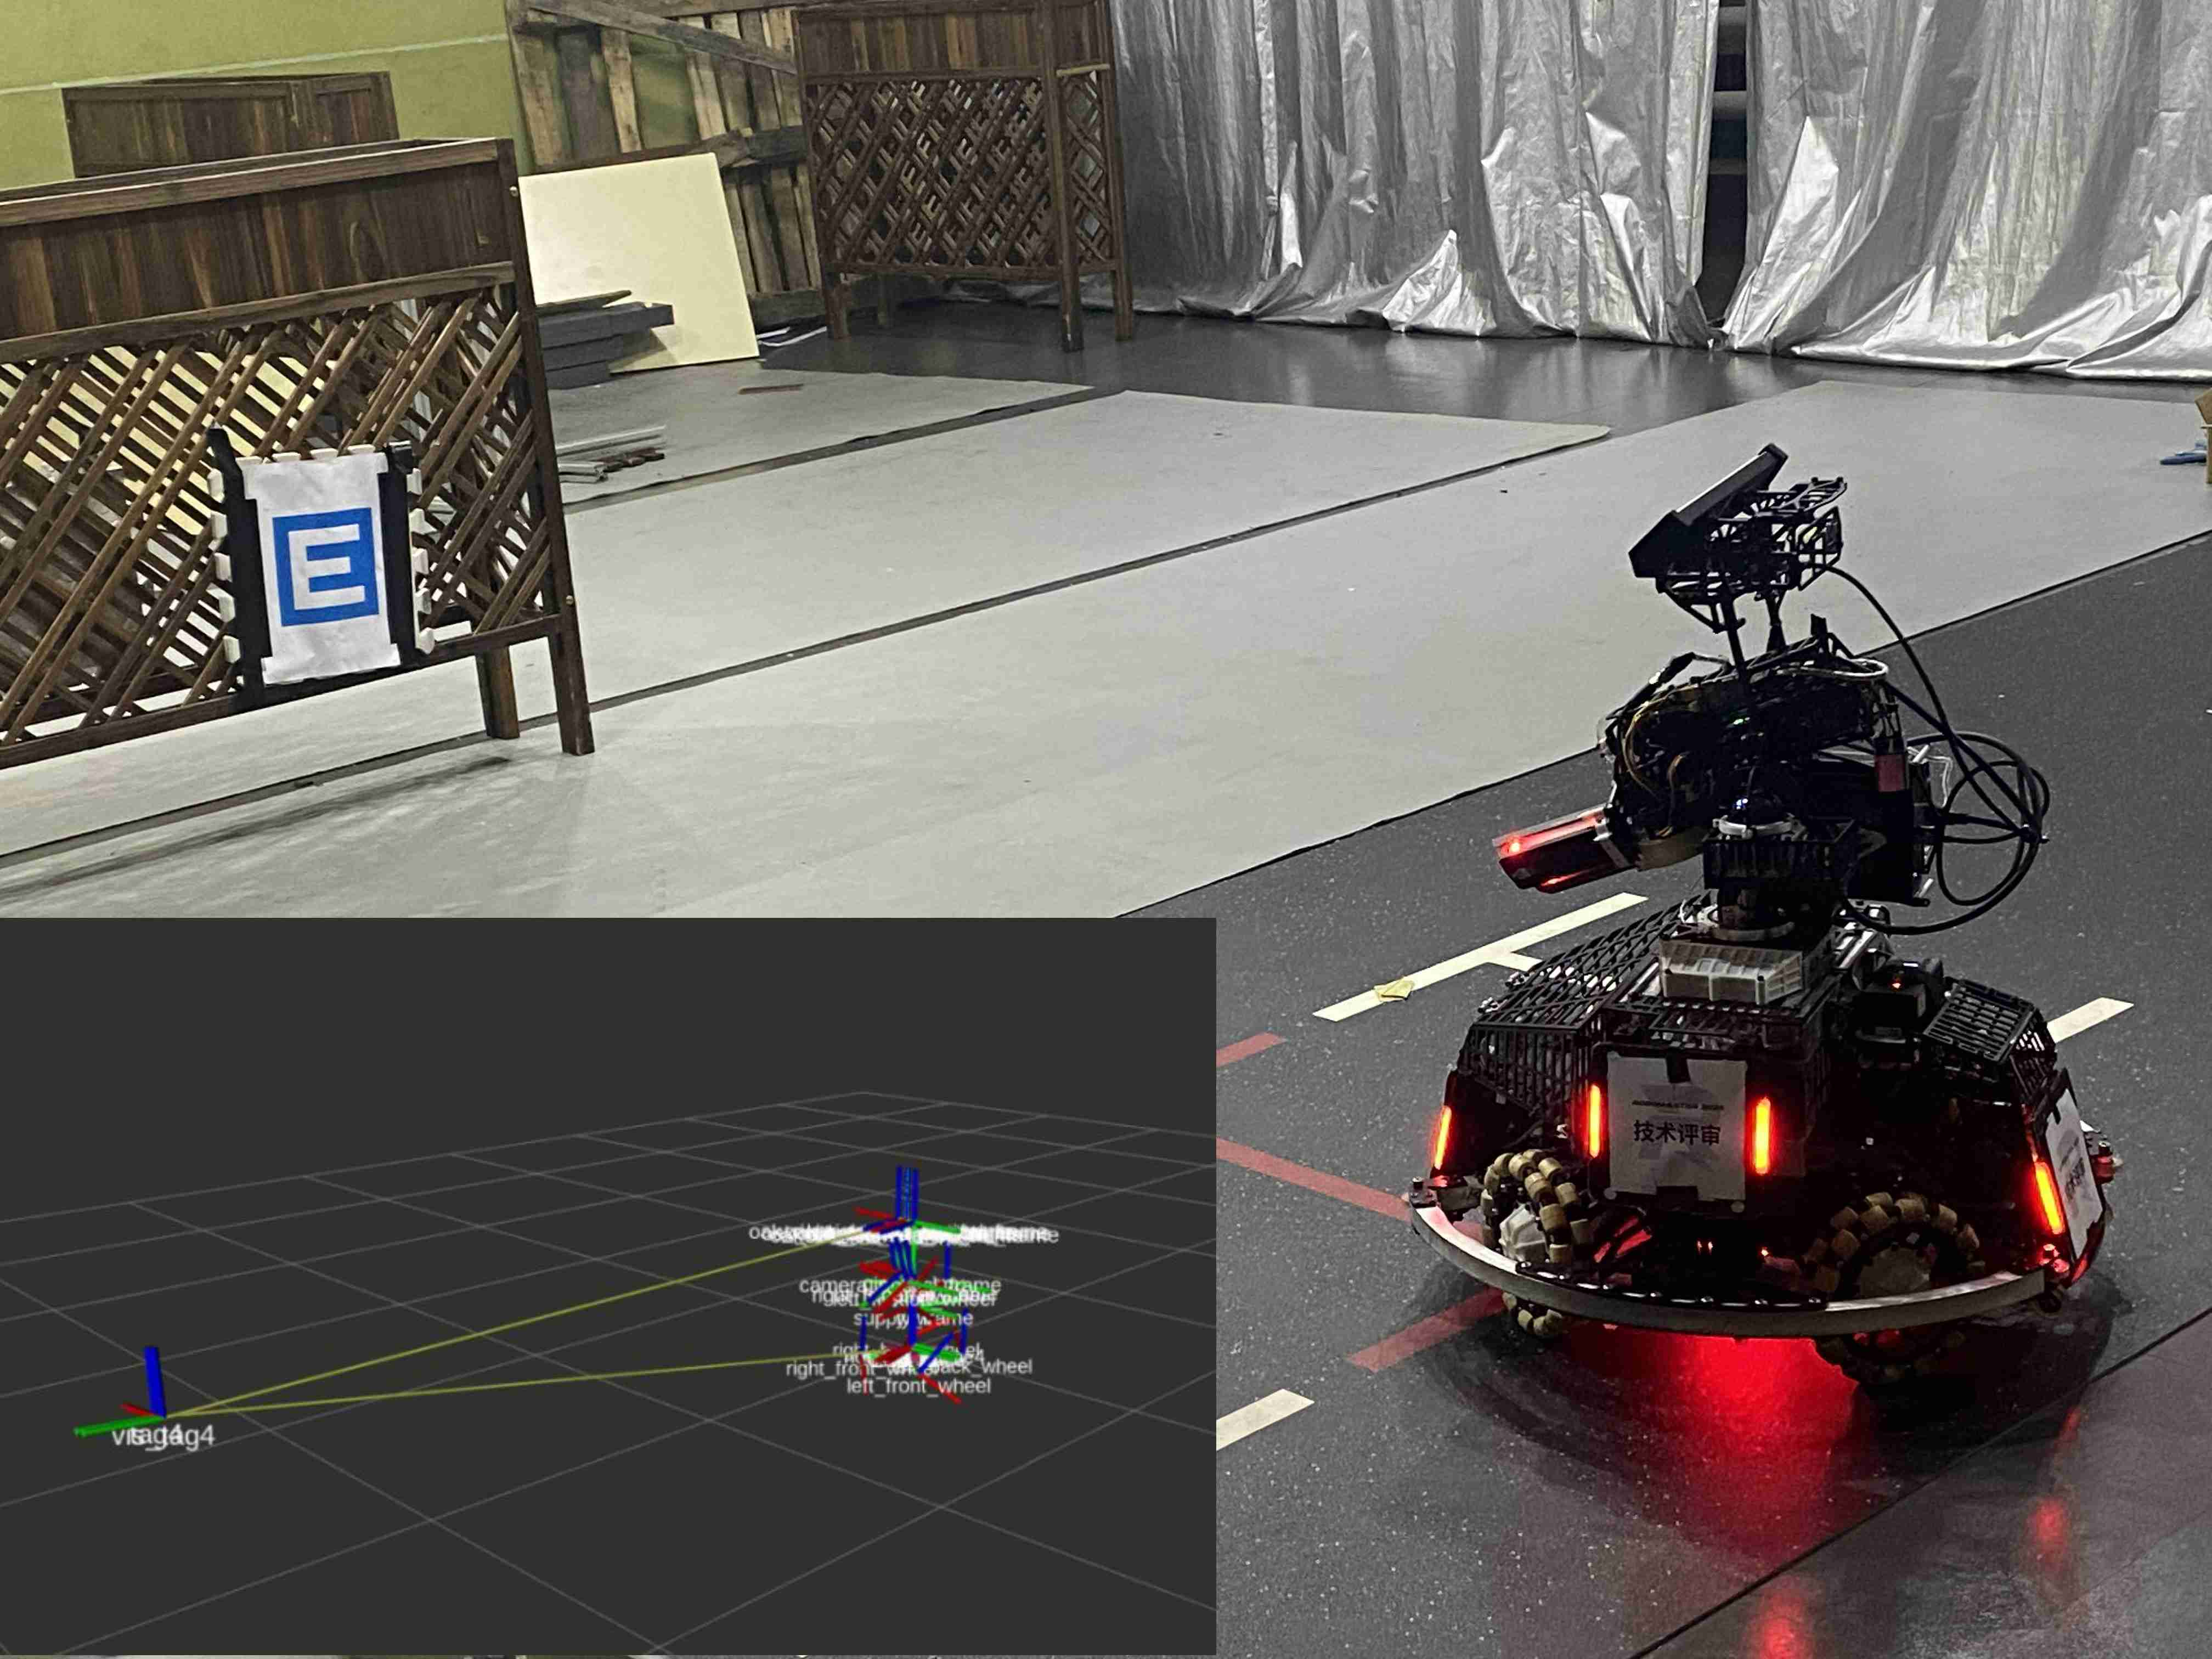
\includegraphics[width=0.5\columnwidth]{figure/设计方案/定位与导航/视觉标签修复定位.jpg}
    \caption{视觉标签修复效果}
    \label{fig:视觉定位标签修复}
\end{figure}

\paragraph{通过雷达机器人给出的位姿信息修复}
由于赛场环境复杂，以及算法难免产生误差，为了能够人为的修正机器人的位姿，我们同时使用了雷达机器人提供的哨兵位姿信息来修复\lstinline{map -> odom}，考虑到裁判系统在赛场中的通信延迟，我们并不实时的根据雷达机器人的信息去修正坐标，而是在哨兵位置漂移较大的时候让机器人静止，使用雷达机器人发布的哨兵位姿信息覆盖原先的位姿。


\subsubsection{局部定位}
因为赛场上环境复杂，轮式里程计很容易发生漂移，因此局部定位我们采用雷达里程计的信息去修复轮式，通过 \lstinline{FAST_LIO} 发布的里程计信息，我们可以获取雷达相对于上电时姿态的变化 ${}^{lidar}T_{world}$, 以及轮式里程计坐标系到雷达坐标系的相对位姿关系　${}^{odom}T_{lidar}$，据此我们可以计算出雷达初次上电时的坐标系相对与哨兵轮式里程计的位姿态关系 ${}^{world}T_{odom}$ .该关系仅计算一次，即雷达上电后${}^{world}T_{odom}$ 关系保持不变。而后借由雷达与哨兵的位姿关系${}^{lidar}T_{base}$,以及 \lstinline{FAST_LIO} 发布的雷达相对上电姿态的关系${}^{lidar}T_{world}$，得出里程计坐标系到机器人底盘坐标系的关系：
\begin{equation}
    {}^{odom}T_{base} = {}^{odom}T_{world}  {}^{world}T_{lidar} {}^{lidar}T_{base} 
\end{equation}

计算出哨兵的里程计信息，以此替换原先的轮式里程计。

\subsection{点云处理}
由于雷达的安装问题以及场地环境的复杂，雷达会产生机器人身体或者不适合规划的点云，因此我们采用了开源工具 \lstinline{robot_body_filter} 来滤除根据机器人身体产生的点云，同时使用 \lstinline{pcl_ros} 中的滤波器对点云进行高度滤波以及去除雷达中的离散点。
